\chapter{Root Finding}
\label{Ch: 0-Ro-Fi}

Root finding is a fundamental problem in numerical analysis and has many applications in science and engineering such as solving nonlinear equations, optimization problems, and differential equations. Usually, a closed form of the root is not available, and we need to compute the root numerically. In this chapter, we will discuss some of the most common methods for root finding.

\section{Bracket Methods}
\label{Sec: 0-Br-Me}

If $f$ is a continuous function, and $f(a)$ and $f(b)$ have opposite signs, then by the Intermediate Value Theorem, there exists a root of $f$ on the interval $[a, b]$. The bracket method is based on this fact and iteratively locates the pair of points $a$ and $b$ such that $f(a)$ and $f(b)$ have opposite signs. The most common bracket methods are the bisection method and the false position method.

\subsection{Bisection Method}
\label{SSec: 0-Bi-Me}

The simplest bracket method is the bisection method. Once $f(a)f(b) < 0$, one can select the midpoint $c = \frac{a + b}{2}$ and check the sign of $f(a) f(c)$.

\begin{itemize}
    \item If $f(a)f(c) < 0$, then the root is in the interval $[a, c]$.
    \item If $f(a)f(c) > 0$, then the root is in the interval $[c, b]$.
    \item If $f(a)f(c) = 0$, then $c$ is the root.
\end{itemize}

For the first two cases, we can repeat the process with the new interval until certain stop criteria are met. Each iteration reduces the size of the interval by half (gaining one bit each iteration), and the total number of iterations required to reduce the interval to a certain size is $\lceil\log_2\left(\frac{b - a}{\epsilon}\right)\rceil$, where $\epsilon$ is the desired tolerance.

Once the function $f$ has a sign change over the bracket $[a, b]$, the bisection method is guaranteed to converge to a root, but it is not very efficient. It is usually used to obtain a rough estimate of the root, which is then taken as an initial guess for a more efficient method.

\begin{remark}
The bisection method can be implemented either iteratively or recursively. The recursive program is usually more compact but may suffer from inefficiency (more instructions) and the risk of stack overflow.

For a variety of programming languages, recursive implementation can be made more efficient by using the so-called tail recursion optimization. This compiler feature allows the recursive program to be executed with the same efficiency as the iterative one. However, neither \texttt{Python} nor \texttt{MATLAB} natively supports tail recursion optimization.
\end{remark}

\subsection{False Position Method}
\label{SSec: 0-Fa-Po-Me}
The bisection method only uses $\text{sgn}(f(a))$ and $\text{sgn}(f(b))$ instead of the function values. The false position method (\emph{Regula falsi} in Latin) improves the bisection method by taking the function values into account. Instead of selecting the midpoint $c = \frac{a + b}{2}$, the false position method selects the point $c\in[a, b]$ that lies on the line connecting $(a, f(a))$ and $(b, f(b))$, that is

$$c = \frac{f(b) a - f(a) b}{f(b) - f(a)} = a - f(a)\frac{b - a}{f(b) - f(a)}.$$

The false position method is also guaranteed to converge to a root if $f(a)f(b) < 0$ and the implementation is quite similar to the bisection method. It usually converges faster than the bisection method, but sometimes exceptions occur.

\begin{remark}
    When $f''$ keeps the same sign over $[a, b]$, it is not hard to show that only one side of the bracket is updating. The bracket size will never decrease to zero, which is different from the bisection method. In the following, we use an example to illustrate this, see Figure~\ref{FIG: 0-RO-FI-FA}. The function $f(x) = x^2 - 1$ over the initial bracket $[0, 2]$. The left endpoint is updating to the root while the right endpoint is fixed at $2$.

\begin{figure}[!htb]
    \centering
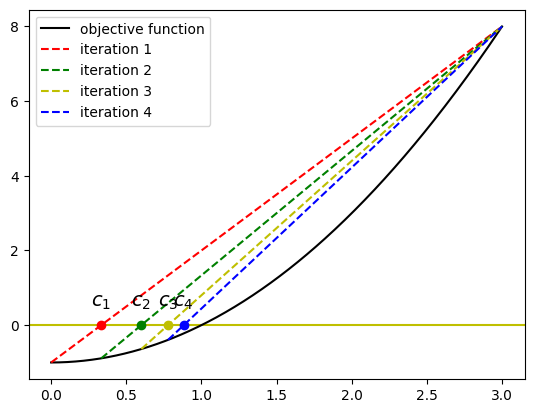
\includegraphics[scale=0.6]{Figures/root_finding_img_0.png}
    \caption{False position method}
    \label{FIG: 0-RO-FI-FA}
\end{figure}
\end{remark}

It is easy to improve the false position method by forcing more weight toward the other endpoint. This is called the Illinois method. Once the same side has updated in two consecutive iterations, the Illinois method will adjust $c$ using a slightly different formula.

$$
{c} = a - f(a)\frac{ b - a }{\lambda f(b) - f(a)}
\quad \text{or}\quad 
{c} =  b -  f(b) \frac{a - b}{\lambda f(a) - f(b)},
$$

where the weight $\lambda$ controls the position of $c$. The weight is initially set to $1$ which corresponds to the standard false position method. If the same side is about to update twice, the weight of the other side will be halved. If not, the weight on the new bracket point will be reset to $1$. See Algorithm~\ref{ALG: ILLINOIS}.

\begin{algorithm}[!htb]
    \SetAlgoLined
    \caption{Illinois Method}
    \KwData{$f$, $a, b$, $\epsilon$}
    \KwResult{root $c$}
    $x_0\gets a$
    
    $x_1\gets b$
    
    $f_0\gets f(x_0)$
    
    $f_1\gets f(x_1)$
    
    $iter = 0$ //    initialization; 
    \\
    \While{\texttt{True}}{
       $x_2 \gets x_0 - f_0 \frac{x_1 - x_0}{f_1 - f_0}$
       
       $f_2 \gets f(x_2)$
       
       $iter \gets iter + 1$. //standard false position step;
       
        \If{$ |f_2| < \epsilon$}{ return $x_2$ //check stopping criteria; }
        \While{$f_1 f_2 > 0$}{

        $(x_0, f_0)\gets (x_0, \lambda f_0)$, where $\lambda = \frac{1}{2}$
        
        $(x_1, f_1)\gets (x_2, f_2)$ 
        
        $x_2 \gets x_0 - f_0 \frac{x_1 - x_0}{f_1 - f_0}$
        
        $f_2 \gets f(x_2)$
        
        $iter \gets iter + 1$.

        \If{$ |f_2| < \epsilon$ }{return $x_2$; //check stopping criteria;}
        }
        \If {$f_1 f_2 < 0$}{ $(x_0, f_0)\gets (x_1, f_1)$ 
        
        $(x_1, f_1)\gets (x_2, f_2)$. }
        
    }
    \label{ALG: ILLINOIS}
\end{algorithm}


\begin{remark}
The choice of decay factor $\frac{1}{2}$ is optimal if it has to be a constant (explain later). The factor can be replaced with other variable values. A usual replacement is the Pegasus method.

Essentially, the Pegasus method replaces $\lambda = 1/2$ with $\lambda=\frac{f_1}{f_1 + f_2}$.

\end{remark}

\begin{remark}
We use the previous example to illustrate the difference between the false position method and the Illinois method. At the second iteration, the Illinois method finds the updating is still on the left side, so it modifies the right endpoint $f(b)$ into $\frac{1}{2} f(b)$ to compute the new $c$, which makes the selected point ${c}$ closer to the right endpoint than the false position method, see Figure~\ref{FIG: 0-RO-FI-IL}.

\begin{figure}[!htb]
    \centering
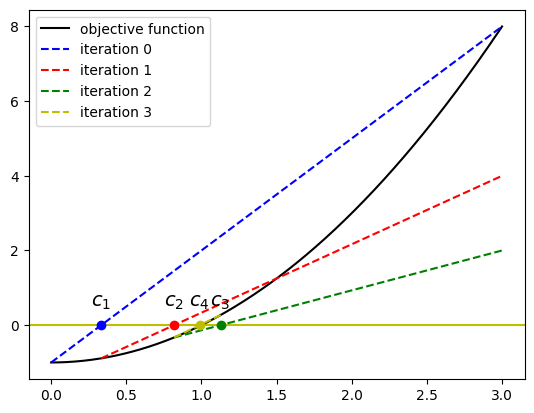
\includegraphics[scale=0.6]{Figures/root_finding_img_1.png}
    \caption{Illinois method}
    \label{FIG: 0-RO-FI-IL}
\end{figure}
\end{remark}

\begin{remark}
    The bracket methods need to first locate an interval $[a, b]$ such that $f(a)f(b) < 0$. A common approach is to sample a few equidistant points in a large interval and then use the sign of the function values to identify the bracket. This is a simple and robust approach, but it may require a large number of function evaluations.
\end{remark}

\subsection{Order of Convergence}
The order of convergence quantifies how fast the sequence approximates the limiting value.

\begin{definition}
The order of convergence of a sequence $\{x_n\}$ is $p > 0$ if 
$$
\lim_{n\to\infty}\frac{|x_{n+1} - x^{\ast}|}{|x_n - x^{\ast}|^p} = \rho,
$$
The constant $\rho$ is the rate of convergence. If $p = 1$, the sequence is said to have linear convergence. If $p = 2$, the sequence is said to have quadratic convergence. 
If the limit does not exist while the upper bound exists for sufficiently large $n$:
$$
\frac{|x_{n+1} - x^{\ast}|}{|x_n - x^{\ast}|^p} \le \rho,
$$
then the order of convergence is at least $p$ and the rate of convergence is at most $\rho$.
\end{definition}
\begin{remark}
   In practice, the limit or even upper bound may not exist for $\frac{|x_{n+1} - x^{\ast}|}{|x_n - x^{\ast}|^p}$, it is possible to consider the convergence rate in a weaker sense. For instance, for sufficiently large $n$ that the inequality 

$$
\lim_{k\to\infty}\sqrt[k]{\frac{|x_{n+k} - x^{\ast}|}{|x_n - x^{\ast}|^{p^k}}}= \rho
$$

holds for certain $p > 0$ and $\rho > 0$, then the sequence has a mean order of convergence is $p$ and a mean convergence rate $\rho$. On average, each iteration contributes an order of $p$ and a rate of $\rho$. 
\end{remark}

\begin{theorem}
The bisection method has a linear convergence rate.   
\end{theorem}

\begin{proof}
Without loss of generality, we may assume the initial bracket is on $[0, 1]$. Let the root $x^{\ast} = 0.b_1 b_2\cdots$ be the binary representation, then the sequence of bisection method can be written as 
$$
x_n = 0.b_1 b_2\cdots b_{n-1} 1,
$$
where $b_i$ is the $i$-th bit of the binary representation. The error at the $n$-th iteration is
$$|x_n - x^{\ast}| = |2^{-n} - \sum_{j\ge n} 2^{-j} b_j|=\begin{cases}\sum_{j>n} 2^{-j}b_j & \text{if } b_n=1\\\sum_{j>n} 2^{-j}(1-b_j) &\text{if }b_n=0\end{cases}$$
For each $n$ such that $b_n = 1$ (similar argument holds for $b_n=0$), we can find $s\in\mathbb N$ such that $b_{s+n} = 1$, otherwise we arrive at the exact solution. 
$$
\frac{|x_{n+k} - x^{\ast}|}{|x_n - x^{\ast}|} = \frac{\sum_{j>n+k} 2^{-j} b_j }{\sum_{j>n} 2^{-j}b_j} \le \frac{2^{-(n+k)}}{2^{-(n+s)}} =2^{s - k} $$
Therefore, the geometric mean of the convergence rate is bounded by $\frac{1}{2}$.
$$
\rho =\lim_{k\to\infty} \sqrt[k]{\frac{|x_{n+k} - x^{\ast}|}{|x_n - x^{\ast}|}} \le \lim_{k\to\infty}2^{s/k}\frac{1}{2} =\frac{1}{2}.
$$
\end{proof}


A common technique to study the order of convergence is to use the Taylor expansion. Let us use the Illinois method as an example.

\begin{theorem}
\label{THM: 0-IL-ME}
    The order of convergence of the Illinois method is $\sqrt[3]{3}$.
\end{theorem}

\begin{proof}
Let $f(x)\in C^2[a, b]$ and $x^{\ast}$ be the root. For simplicity, we assume the root is simple. Let $\ell(x)$ be the linear interpolation of $f$ at the bracket $[a, b]$, the slope is $f'(\zeta)=\frac{f(b) - f(a)}{b -a}$, then 

$$
f(x) - \ell(x) = \frac{f''(\xi)}{2}(x - a)(x - b),
$$
therefore, the root satisfies $-\ell(x^{\ast}) = \frac{f''(\xi)}{2}(x^{\ast} - a)(x^{\ast} - b)$. Let $c$ be the next iteration, then 

$$
-\ell(x^{\ast}) + \ell(c) = -(x^{\ast} - c) f'(\zeta) =  \frac{f''(\xi)}{2}(x^{\ast} - a)(x^{\ast} - b),
$$

which implies $(x^{\ast} - c) = -\frac{f''(\xi)}{2 f'(\zeta)} (x^{\ast} - a)(x^{\ast} - b)$. When $a$ and $b$ are already near the root, the right-hand side has a fixed sign, which implies that using the unadjusted false position method, the new point $c$ will always fall into a fixed side of the root.

Now, we consider the adjustment of the Illinois method. Without loss of generality, we assume that $c$ falls into the left side of the root. Then the next iteration will be using the bracket $[c, b]$ with adjusted weight for $b$. The new point $c'$ satisfies 

$$
\begin{aligned}
c' - x^{\ast} &= \frac{\frac{1}{2} f(b) (c - x^{\ast}) - f(c) (b - x^{\ast})}{\frac{1}{2} f(b) - f(c)}  = (c - x^{\ast}) - \frac{f(c)(b-x^{\ast})}{\frac{1}{2}f(b) - f(c)}
+ \frac{f(c)(c - x^{\ast})}{\frac{1}{2}f(b) - f(c)}\\
&= (c - x^{\ast}) - \frac{2f(c)}{f(b)}(b - x^{\ast}) \frac{1}{1 - \frac{2f(c)}{f(b)}} + \frac{2f(c)}{f(b)}(c - x^{\ast}) \frac{1}{1 - \frac{2f(c)}{f(b)}}
\end{aligned}
$$

Using Taylor expansion at $x^{\ast}$, since $f'$ is bounded from below near the root, 

 $$
 \begin{aligned}
 \frac{f(c)}{f(b)} &= \frac{(c - x^{\ast}) + \cO(|c - x^{\ast}|^2)}{(b - x^{\ast}) + \cO(|b - x^{\ast}|^2)} = \frac{(c - x^{\ast})}{(b - x^{\ast})}\left(1 + \frac{\cO(|b-x^{\ast}|) + \cO(|c - x^{\ast}|)}{1 + \cO(|b-x^{\ast}|)}\right) \\&= \frac{(c - x^{\ast})}{(b - x^{\ast})}\left(1 + \cO(|b-x^{\ast}|)\right) = \frac{f''(\xi)}{2 f'(\zeta)} (a - x^{\ast}) \left(1 + \cO(|b-x^{\ast}|)\right)  .
 \end{aligned}
 $$ 

Therefore, we obtain

$$
\begin{aligned}
c' - x^{\ast} &= (c- x^{\ast}) + 2(x^{\ast} - c)\left(1 + \cO(|a - x^{\ast}|)\right) + \cO(|a - x^{\ast}||c - x^{\ast}|) \\
&= (x^{\ast} - c)(1 + \cO(|a - x^{\ast}|)),
\end{aligned}
$$
which moves the new point to the other side of the root by almost reflection. The next bracket becomes $[c, c']$ such that $|c - x^{\ast}|\approx |c' - x^{\ast}|$. Therefore, if denote the last two points as $c = x_{n}$ and $c'=x_{n+1}$, then $|x_{n} - x^{\ast}|\approx |x_{n+1} - x^{\ast}|$, currently $c'$ is on the right side of the root. The next three iterations satisfy

\begin{itemize}
    \item  $|x_{n+2} - x^{\ast}| = \Theta(|x_n - x^{\ast}| |x_{n+1} - x^{\ast}|) = \Theta(|x_{n+1} - x^{\ast}|^2) $, the iteration $x_{n+2}$ is on left side.
    \item  $|x_{n+3} - x^{\ast}| = \Theta(|x_{n+2} - x^{\ast}||x_{n+1} - x^{\ast}|) = \Theta(|x_{n+1} - x^{\ast}|^3)$, the iteration $x_{n+3}$ is again on left side.
    \item  $|x_{n+4} - x^{\ast}| = \Theta(|x_{n+3} - x^{\ast}|) = \Theta(|x_{n+1} - x^{\ast}|^3)$, adjusted by Illinois method, the iteration $x_{n+4}$ is on right side, which completes a cycle.
\end{itemize}

By the previous definition of order of convergence, the Illinois method has an order of convergence $\sqrt[3]{3}$.
\end{proof}

\begin{remark}
\label{REM: 0-CO-IL-AS}
A quick way of proof uses the asymptotic analysis. 

If we denote $\epsilon_{n} =x_n - x^{\ast}$, then if $\epsilon_{i} > 0$ and $\epsilon_{i-1} < 0$, then $\epsilon_{i+1} \simeq C \epsilon_{i}\epsilon_{i-1}$, where $C\approx \frac{f''(x^{\ast})}{2f'(x^{\ast})}$, here we may assume $C > 0$, then $\epsilon_{i+1} < 0$.  The next iteration applies the same rule, which is $\epsilon_{i+2} \simeq C \epsilon_{i+1}\epsilon_{i} = C^2 \epsilon_i^2 \epsilon_{i-1} < 0$.  Now, we need an adjustment step, which gives $\epsilon_{i+3} = -C^2 \epsilon_i^2 \epsilon_{i-1} > 0$, which completes a cycle. Every three iterations make a cycle, to derive the order of convergence, we continue to derive $\epsilon_{i+6}$, which equals to $-C^8\epsilon_{i}^6\epsilon_{i-1}^3 = C^2\epsilon_{i+3}^3$. Therefore, the order of convergence is $\sqrt[3]{3}$.
\end{remark}

By taking the decay factor as a constant, the order of convergence is at most $\sqrt[3]{3}$. However, if the decay factor can be chosen as a variable one, the order of convergence can be improved. Next, we apply the same technique to analyze the Pegasus method, which is a variant of the Illinois method. Interestingly, the Pegasus method was initially discovered in a subroutine for the Ferranti Pegasus computer, but no author information is included. The convergence analysis was given by~\cite{dowell1972pegasus} after its discovery.

\begin{theorem}
    \label{THM: 0-PE-ME}
The Pegasus method is a variant of the Illinois method, whose updating scheme for the decay factors is replaced by 

$$\lambda=\frac{f_1}{f_1+f_2}$$ 

in {prf:ref}`AL-ILLINOIS`. Then the order of convergence is $\sqrt[4]{\frac{7+\sqrt{57}}{2}}$.    
\end{theorem}

\begin{proof}
Similar to the previous Remark~\ref{REM: 0-CO-IL-AS}, we assume $\epsilon_{i-1} < 0$ and $\epsilon_{i} > 0$ such that $|\epsilon_i|\ll |\epsilon_{i-1}|$, the constant $C = \frac{f''}{2f'}|_{x=x^{\ast}} > 0$.
Similar to the previous analysis, we can derive more terms in the asymptotic form
$$
\epsilon_{i+1}\simeq C \epsilon_{i}\epsilon_{i-1} + D \epsilon_{i} \epsilon_{i-1}(\epsilon_{i} + \epsilon_{i-1})< 0
$$
where $D = -C^2 + \frac{f'''}{6f'}|_{x=x^{\ast}}$. Then due to a different sign for $\epsilon_{i}$ and $\epsilon_{i+1}$, we can derive 
$$\epsilon_{i+2}\simeq C \epsilon_{i+1}\epsilon_{i} + D \epsilon_{i+1} \epsilon_{i}(\epsilon_{i+1} + \epsilon_{i}) < 0.$$
Now use the adjustment step, we obtain (needs some calculation)
$$
\begin{aligned}
\epsilon_{i+3} &= \frac{\epsilon_{i+2}\lambda f(x_i) - \epsilon_i f(x_{i+2})}{\lambda f(x_{i}) - f(x_{i+2})},\quad \lambda = \frac{f(x_{i+1})}{f(x_{i+2}) + f(x_{i+1})}\\
&\approx C^2 \epsilon_{i}^2\epsilon_{i+2} - D \epsilon_{i} \epsilon_{i+1} \epsilon_{i+2}, 
\end{aligned}
$$
it implies $\epsilon_{i+3} < 0$ as well. Therefore, another adjustment step is needed (after some more calculations, see Remark~\ref{REM: 0-CO-PE-AS})
$$
\begin{aligned}
\epsilon_{i+4} &=  \frac{\epsilon_{i+3}\lambda f(x_i) - \epsilon_i f(x_{i+3})}{\lambda f(x_{i}) - f(x_{i+3})},\quad \lambda = \frac{f(x_{i+2})}{f(x_{i+3}) + f(x_{i+2})}\frac{f(x_{i+1})}{f(x_{i+2}) + f(x_{i+1})}\\
&\approx C^5 \epsilon_{i}^4\epsilon_{i+1}^2 > 0.
\end{aligned}
$$
Therefore, $\epsilon_{i+4}\approx C \epsilon_{i+3} \epsilon_{i+2}$. A full cycle consists of 4 iterations and 
$$
\epsilon_{i+8} \simeq C^7 \epsilon_{i+4}^6 \epsilon_{i+3}^2 \simeq C^{8}\epsilon_{i+4}^7 \epsilon_i^2.
$$
The order of convergence $p$ solves $p^2 - 7p - 2 = 0$, which gives $p = \sqrt[4]{\frac{7+\sqrt{57}}{2}}$.
\end{proof}

\begin{remark}
\label{REM: 0-CO-PE-AS}
Actually, the asymptotic expansion of $\epsilon_{i+4}$ is (expanded in $\epsilon_{i+1}$ first )

$$
\epsilon_{i+4} = C^5 \epsilon_{i}^4\epsilon_{i+1}^2 + C^7 \epsilon_i^7\epsilon_{i+1}
+ \cO(\epsilon_{i}^8 \epsilon_{i+1} + \epsilon_{i}^5 \epsilon_{i+1}^2 + \epsilon_{i}^3 \epsilon_{i+1}^3)$$

It is at first not clear why we can retain the first term and drop the rest because it requires the following inequalities to hold

$$\epsilon_{i}^3 \ll \epsilon_{i+1}\ll \epsilon_i.$$

The latter one is correct because of the relation $\epsilon_{i+1} \simeq C \epsilon_{i}\epsilon_{i-1} \ll \epsilon_i$ once the iterations are close to the root. The former one is equivalent to $\epsilon_{i}^2 \ll \epsilon_{i-1}$. This can be made into an assumption because $\epsilon_{i-1}$ and $\epsilon_{i}$ are the last two iterations in the previous cycle, which correspond to $\epsilon_{i+3}$ and $\epsilon_{i+4}$ in the current cycle, we can use the above asymptotic estimate to find $\epsilon_{i+3}^3 \approx C^6 \epsilon_{i}^9 \epsilon_{i+1}^3 \ll \epsilon_{i+4}$. 

Therefore, if the inequality does not hold, one can use the current cycle as the starting point to perform the same analysis.
\end{remark}

In the Pegasus method, two consecutive standard false position steps and two adjustment steps are performed in a full cycle. Although the decay over a full cycle is significant, such an advantage will be gone if the cycle is long. To make the cycle shorter, we need to drop at least one step. According to the previous analysis (see Illinois method), the standard false position step does not change the sign of the error asymptotically, thus it is preferred to drop one of the standard false position steps.

Let us finish this section with a brief discussion on the improved Pegasus method \cite{king1973improved}, which takes advantage of the symmetry in the false position method to avoid consecutive standard false position steps. A similar technique can be also applied to other methods such as the Anderson-Bjorck method \cite{anderson1973new}.

\begin{algorithm}[!htb]
    \SetAlgoLined
    \caption{Improved Pegasus Method}
    \KwData{$f$, $a, b$, $\epsilon$}
    \KwResult{root $c$}
    $x_0\gets a$
    
    $x_1\gets b$
    
    $f_0\gets f(x_0)$
    
    $f_1\gets f(x_1)$
    
    $iter = 0$ //    initialization; 
    \\
    \While{\texttt{True}}{
       $x_2 \gets x_0 - f_0 \frac{x_1 - x_0}{f_1 - f_0}$
       
       $f_2 \gets f(x_2)$
       
       $iter \gets iter + 1$. //standard false position step;
       
        \If{$ |f_2| < \epsilon$}{ return $x_2$ //check stopping criteria; }
        {\color{cyan}\If{$f_1 f_2 < 0$}{swap $(x_0, f_0)$ and $(x_1, f_1)$; // avoid false position step}}
        \While{$f_1 f_2 > 0$}{

        $(x_0, f_0)\gets (x_0, \lambda f_0)$, where $\lambda = \frac{1}{2}$
        
        $(x_1, f_1)\gets (x_2, f_2)$ 
        
        $x_2 \gets x_0 - f_0 \frac{x_1 - x_0}{f_1 - f_0}$
        
        $f_2 \gets f(x_2)$
        
        $iter \gets iter + 1$.

        \If{$ |f_2| < \epsilon$ }{return $x_2$; //check stopping criteria;}
        }
        \If {$f_1 f_2 < 0$}{ $(x_0, f_0)\gets (x_1, f_1)$ 
        
        $(x_1, f_1)\gets (x_2, f_2)$. }
        
    }
    \label{ALG: IMPROVE_PEGASUS}
\end{algorithm}

\begin{theorem}
The improved Pegasus method has an order of convergence at least $\sqrt[3]{5}$.
\end{theorem}
\begin{proof}
In the same setting as the previous theorem, we will find the first iteration is the same as the Pegasus method (false position) that
$$\epsilon_{i+1}\simeq C \epsilon_i \epsilon_{i-1} + D \epsilon_i \epsilon_{i-1}(\epsilon_{i} + \epsilon_{i-1}) < 0.$$
For the second iteration, although $x_{i+1}$ and $x_{i}$ are on different sides, a false position step has been performed in the previous step, thus it will perform an adjustment step with $\lambda = \frac{f(x_{i}) - f(x_{i+1})}{f(x_{i})}$, then
$$\epsilon_{i+2} \simeq -D \epsilon_{i+1}\epsilon_{i}\epsilon_{i-1},$$
note the leading term is different from the Pegasus method. There are two options.
\begin{itemize}
    \item If $D < 0$, then $\epsilon_{i+2} > 0$ which completes a cycle with two iterations, which is very compact. In this case, we find
    $$\epsilon_{i+4} \simeq C^{2}  \epsilon_{i+2}^3,$$
    which implies an order of convergence at $\sqrt{3}$.
    \item If $D > 0$, then it will perform another adjustment step,
    $$\epsilon_{i+3} =  \frac{\epsilon_{i+2}\lambda f(x_i) - \epsilon_i f(x_{i+2})}{\lambda f(x_{i}) - f(x_{i+2})},\quad \lambda = \frac{f(x_{i+1})-f(x_{i+2})}{f(x_{i+1})}\frac{f(x_{i})-f(x_{i+1}) }{ f(x_{i})}$$
    which will make $\epsilon_{i+3} \simeq -C^3 D \epsilon_{i-1}^3 \epsilon_i^3 > 0$, which completes a cycle with three iterations. In this case, we find
    $$\epsilon_{i+6} \simeq D^{2}  \epsilon_{i+3}^5,$$
    which implies an order of convergence at $\sqrt[3]{5}$. 
\end{itemize}
\end{proof}

\section{Iterative Methods}
\label{Sec: 0-IT-ME}
In theory, the bracket methods are also iterative. However, one important phenomenon of bracket methods is that the current iteration may not be generated by the latest iterations. For instance, the false position method will have a stalled endpoint once the iterations are near the root. In the following, we will introduce some iterative methods, which generate new iterations based on the latest iterations.

\subsection{Newton-Raphson Method}
Let $f\in C^2$, if the current iteration $x_{n}$ is close to a root, then the Newton-Raphson method computes the next iteration $x_{n+1}$ by

$$
x_{n+1} = x_n - \frac{f(x_n)}{f'(x_n)}.
$$

Geometrically, $x_{n+1}$ is the $x$-intercept of the tangent line of $f$ at $(x_n, f(x_n))$, see Fig~\ref{FIG: 0-RO-FI-NE-ME}. Asymptotically, the Newton-Raphson method has a quadratic convergence rate if the root is simple.

\begin{figure}[!htb]
    \centering
    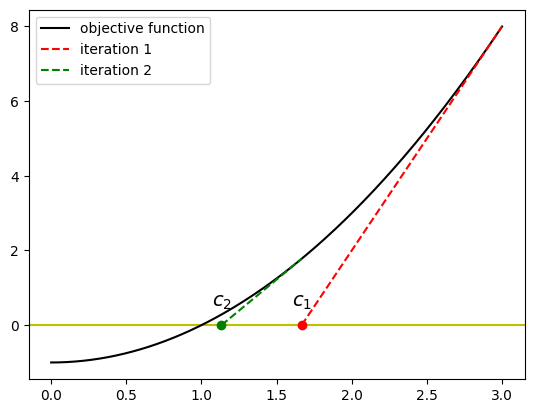
\includegraphics[scale=0.6]{Figures/root_finding_img_2.png}
    \caption{Caption}
    \label{FIG: 0-RO-FI-NE-ME}
\end{figure}

\begin{theorem}
Suppose $f\in C^2$ and the root is simple, then the order of convergence for the Newton-Raphson method is 2.
\end{theorem}
\begin{proof}
The Taylor expansion of $f$ at $x_n$ is
$$f(x) = f(x_n) + f'(x_n)(x - x_n) + \frac{f''(\zeta)}{2}(x - x_n)^2$$
where $\zeta\in (x, x_n)$. The root is $x^{\ast}$, then $f(x^{\ast}) = 0$, thus
$$0 = f(x_n) + f'(x_n)(x^{\ast} - x_n) + \frac{f''(\zeta)}{2}(x^{\ast} - x_n)^2.$$
Therefore,
$$
-\frac{f''(\zeta)}{f'(x_n)} (x^{\ast} - x_n)^2= x^{\ast} - x_n + \frac{f(x_n)}{f'(x_n)} = x^{\ast} - x_{n+1}.
$$
If we denote the error $\epsilon_{n} = x_n - x^{\ast}$, then $\epsilon_{n+1} = \frac{f''(\zeta)}{f'(x_n)} \epsilon_{n}^2$, which implies the order of convergence is 2.
\end{proof}
\begin{remark}
    The analysis can only provide convergence for the initial guess close to the root. If the initial guess is far from the root, then the sequence may diverge.
\end{remark}
\subsection{Secant Method}
\label{SSec: 0-SE-ME}
The secant method is similar to the false position method, but it always uses the latest two iterations to perform the next iteration. The secant method computes the next iteration $x_{n+1}$ by
$$
x_{n+1} = x_n - f(x_n)\frac{x_n - x_{n-1}}{f(x_n) - f(x_{n-1})}.
$$
Using the same derivation for the Illinois method, the error $\epsilon_{n} = x_n - x^{\ast}$ satisfies $\epsilon_{n+1} \simeq C \epsilon_{n}\epsilon_{n-1}$, see Figure~\ref{FIG: 0-RO-FI-SE}.
\begin{figure}[!htb]
    \centering
    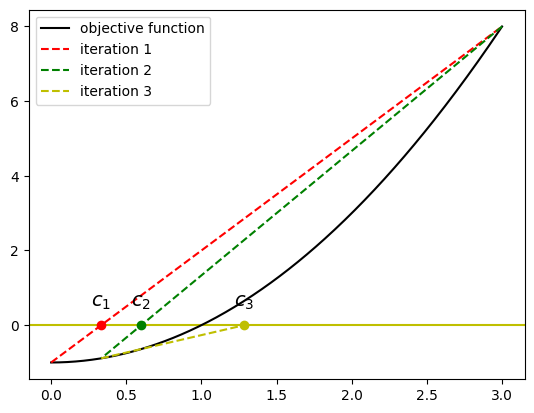
\includegraphics[scale=0.6]{Figures/root_finding_img_3.png}
    \caption{Secant method}
    \label{FIG: 0-RO-FI-SE}
\end{figure}
It is easy to see the order of convergence $p$ solves the equation $p^2 - p - 1 = 0$, which gives $p = \frac{1 + \sqrt{5}}{2}$.
\begin{remark}
    The secant method can be generalized to higher dimensions, which is known as Broyden's method which iteratively updates both the point position and the approximated Jacobian. 
\end{remark}
\subsection{Brent Method}
Brent's method belongs to the class of hybrid methods. It combines the bisection method, secant method, and inverse quadratic interpolation method. 

The inverse quadratic interpolation can be viewed as a generalization of the secant method. Instead of using previous two iterations to generate the next, it uses the three points $(f_{n-2}, x_{n-2})$, $(f_{n-1}, x_{n-1})$, and $(f_{n}, x_{n})$ to find the next iteration at $(0, x_{n+1})$, its formula can be derived easily by 
\begin{equation*}
    x^{n+1} = \frac{f_n f_{n-1}\cdot x_{n-2}}{(f_n - f_{n-2})(f_{n-1} - f_{n-2})}  +  \frac{f_n f_{n-2}\cdot x_{n-1} }{(f_{n} - f_{n-1})(f_{n-2} - f_{n-1})} +  \frac{f_{n-1} f_{n-2}\cdot  x_{n}}{(f_{n-1} - f_{n})(f_{n-2} - f_{n})}.
\end{equation*}
The error $\eps_{n+1}$ can be found by 
\begin{equation*}
    \eps_{n+1} = \frac{f_n f_{n-1} \cdot \eps_{n-2} }{(f_n - f_{n-2})(f_{n-1} - f_{n-2})}  +  \frac{f_n f_{n-2}\cdot \eps_{n-1}  }{(f_{n} - f_{n-1})(f_{n-2} - f_{n-1})} +  \frac{f_{n-1} f_{n-2}\cdot  \eps_{n}}{(f_{n-1} - f_{n})(f_{n-2} - f_{n})}.
\end{equation*}
With the asymptotic expansion $f_n = f'(x^{\ast}) \eps_n + \frac{1}{2} f''(x^{\ast}) \eps_n^2 + \frac{1}{6} f'''(x^{\ast})\eps_n^3 + o(\eps_n^3)$, we can find the leading term is 
$$\eps_{n+1} \approx \left[2 \left(\frac{f''(x^{\ast})}{2f'(x^{\ast})} \right)^2 - \frac{f'''(x^{\ast})}{6f'(x^{\ast})} \right]\eps_{n}\eps_{n-1}\eps_{n-2}.$$
Therefore, the order of convergence $p$ solves $p^3 - p^2 - p - 1 = 0$ which implies $p = \frac{1}{3} + \frac{1}{3}\left(c + \frac{4}{c}\right)\approx 1.83929$, where $c = \sqrt[3]{\frac{38 - \sqrt{1188}}{2}}$. Although the order is greater than secant methods and many other methods, it also has several defects. For instance, if the values $f_n\approx f_{n-1}$ or $f_n\approx f_{n-2}$, the interpolation will be numerically unstable. In such cases, we need to roll back to less effective methods such as secant method.  

\section{Exercises}
\subsection{Theoretical Part}
\begin{problem}
Briefly explain why the formula $x_2 = x_0 - f_0 \frac{x_1 - x_0}{f_1 - f_0}$ in bracket methods will not suffer from catastrophic cancellation when $x_1 - x_0$ is small.
\end{problem}
\begin{problem}
The only difference between the improved Pegasus method and the usual Pegasus method is at the 3rd step in the while loop, which eliminates consecutive false position steps. This change is very simple, but it leads to an improvement in the order of convergence. Explain why the Illinois method $\lambda = \frac{1}{2}$ cannot be faster by the same technique.
\end{problem}
\begin{problem}
Suppose $f\in C^2$ and the root $x^{\ast}$ has a multiplicity of $m>1$, then the order of convergence for the Newton-Raphson method is $1$. The modified Newton-Raphson method
$$
x_{n+1} = x_n - m\frac{f(x_n)}{f'(x_n)}
$$
has an order of convergence $2$.
\end{problem}

\subsection{Computational Part}
\bibliographystyle{apalike}
\bibliography{chap0}